\chapter{Implementation}
\label{cap5}

In this chapter we show how we implemented the Pluto Framework, describing the main elements of the project separately, in order to better understand their behaviors.
In figure \ref{fig:finalArchitecture}, we show the final architecture scheme that includes all the parts described in the following sections.
\\

\begin{figure}[h!]
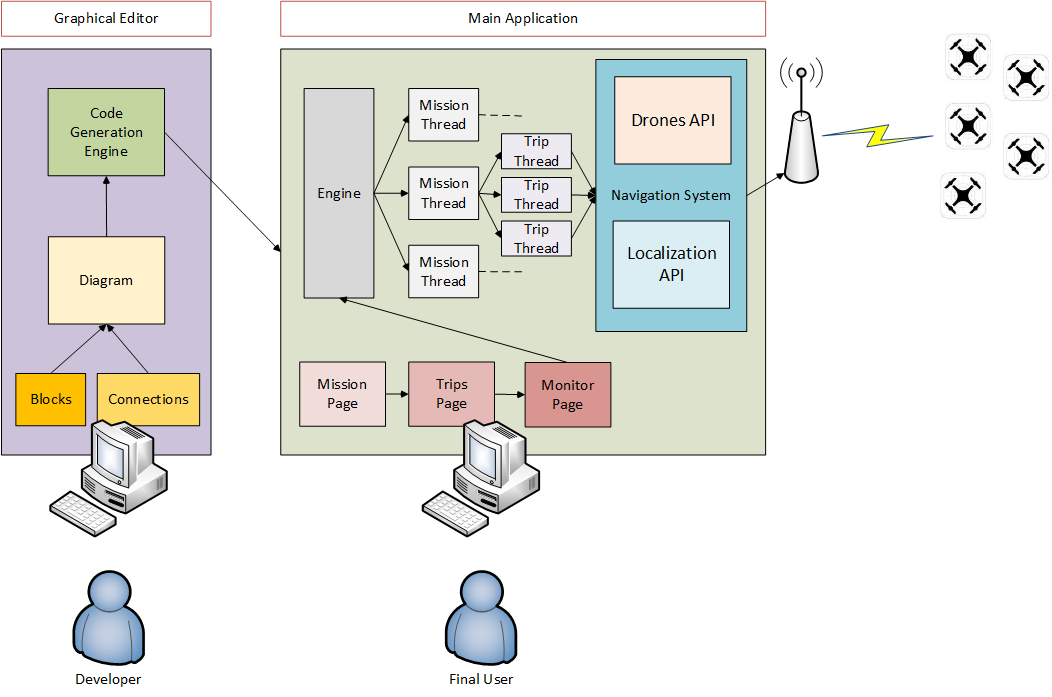
\includegraphics[width=\linewidth]
{pictures/Final_Architecture.png}
\caption{Pluto architecture representation}
\label{fig:finalArchitecture}
\end{figure}

\section{Object-oriented approach}\label{oomodel}

We used the Java programming language to implement both the Graphical Editor and the Main Application.
We made this choice because we are very familiar with Java, since almost every academic project we implemented in these years made use of this Object-Oriented programming language.
The Object-Oriented approach perfectly suits the Pluto model, since we have different independent entities such Drones,Missions,Trips that interact together in the execution of tasks.
\\

We decided to adopt a Model View Controller(MVC) approach.
The central component of MVC, the model, captures the behavior of the application in terms of its problem domain, independent of the user interface.
The model directly manages the data, logic and rules of the application.
A view can be any output representation of information, such as a chart or a diagram; multiple views of the same information are possible.
The third part, the controller, accepts input and converts it to commands for the model or view.
\\

\begin{figure}[h!]
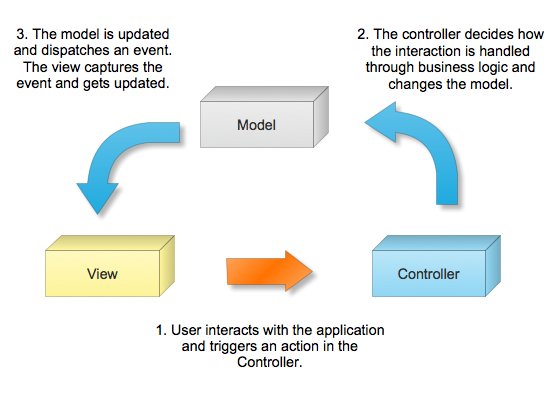
\includegraphics[width=\linewidth]
{pictures/MVC.png}
\caption{MVC design applied to the Main Application}
\label{fig:mvc}
\end{figure}

As shown in figure \ref{fig:mvc}, the model part contains all the Java classes of the entities shown in Section \ref{programmingModel}.
There is a class for the Mission, one for the Trip etc.
The controller part contains the Java classes of all the blocks of the Graphical editor shown in Section \ref{functionalBlocks}.
The controller part also deals with the threads management needed for the execution of both the missions and trips. The thread structure is shown in section \ref{runtimeMng}.
The view part contains the Java classes of the three pages of the Main application shown in Section \ref{plutoMainApp}.
\\

\section{Graphical editor}\label{editor}

In order to create the Graphical Editor, described in section \ref{plutoGraphicalEditor}, we decided to use the GEF (Graphical Editing Framework) project. This framework is a Java technology and it is part of the Eclipse framework developed by IBM.
\\

It gives developers a full solution for the graphical modeling of a Java object model, and it can be used in conjunction with other technologies such as EMF (Eclipse Modeling Framework) or GMF (Graphical Modeling Framework), to enable the creation of a complete graphical modeling suite. 
This means that the Pluto Graphical Editor has been developed as an Eclipse Plugin, so the developer has to install the Eclipse IDE in order to exploit the editor.
\\

First of all, we created the Java classes of all the blocks.
Each class contains the code implementation of the corresponding block, since each block perform a specific functionality.
We defined each block as a rectangle figure, then we added the connection entity in order to enable links between them.
All these entities are children of a main container class that represents the diagram itself that is simply a container for the graph.
Figure \ref{fig:editorExplanation} shows these components: A is the diagram entity, the container of the graph; B is the connection entity, through which the user connects the blocks; C is the block entity. 
\\

\newpage

\begin{figure}[h!]
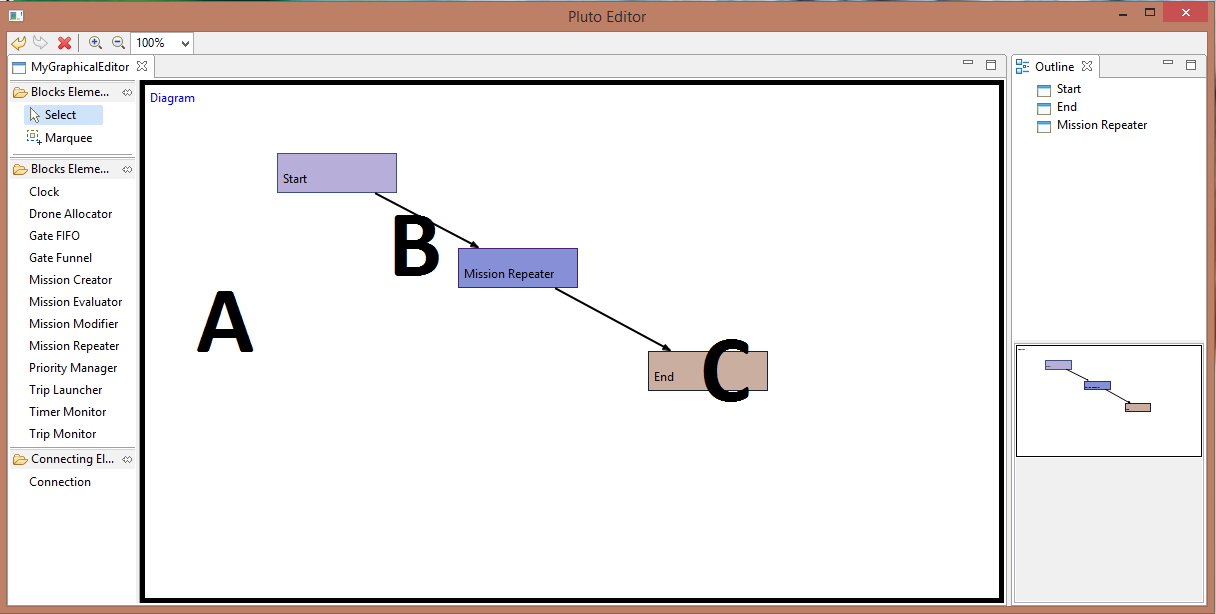
\includegraphics[width=\linewidth]
{pictures/editorExplanation.png}
\caption{Graphical entities in the editor}
\label{fig:editorExplanation}
\end{figure}

When the user creates a new  block in the editor area, a relative block entity is automatically created and added to the diagram container class. The same operation stands for the connections creation.

After the user draws the desired graph he can choose to generate the final code of the Main Application, through the apposite voice in the context menu.
See section \ref{codeGeneration} for further details.
\\

\section{Code generation}\label{codeGeneration}

Once the programmer has created the graph of the application through the Pluto Graphical Editor, he can generate the code in order to make the Pluto Main Application behavior coherent with the graph.

This can be done by right clicking on the graph and choosing the "Generate code" command.

The main issue in the generation process was to understand how to generate the code from a general diagram. 
Potentially, a developer could draw a very complex graph with lot of blocks and connections between them.
At first, we focused on graph exploration methods, but we immediately noticed that they were too complex.
\\

So, we decided to adopt a \textit{Publish-Subscribe} design, making use of the \textit{Observer} pattern. This mechanism let us describe the execution flow of very complex diagrams, besides the more simple ones.
\\
 
The \textit{Observer} pattern consists in the declaration of some elements as \textit{observers} and of other entities as \textit{observable}. 
When an observable object change its status, it sends a notification to all its observer entities. 
These observers will react according to the change of the observable object.
\\

In Figure \ref{fig:observerPattern} there is a sequence diagram that describes how the observer pattern work with a simple diagram with four blocks (A, B, C and D).
\\
The "Observe" message in the sequence is the declaration of a block that wants to observe another block. The "Notify" message represents the notification that a block sends to its observers when it changes its status, or in this case when the blocks ends the management of the Mission object.
\\

 \begin{figure}
 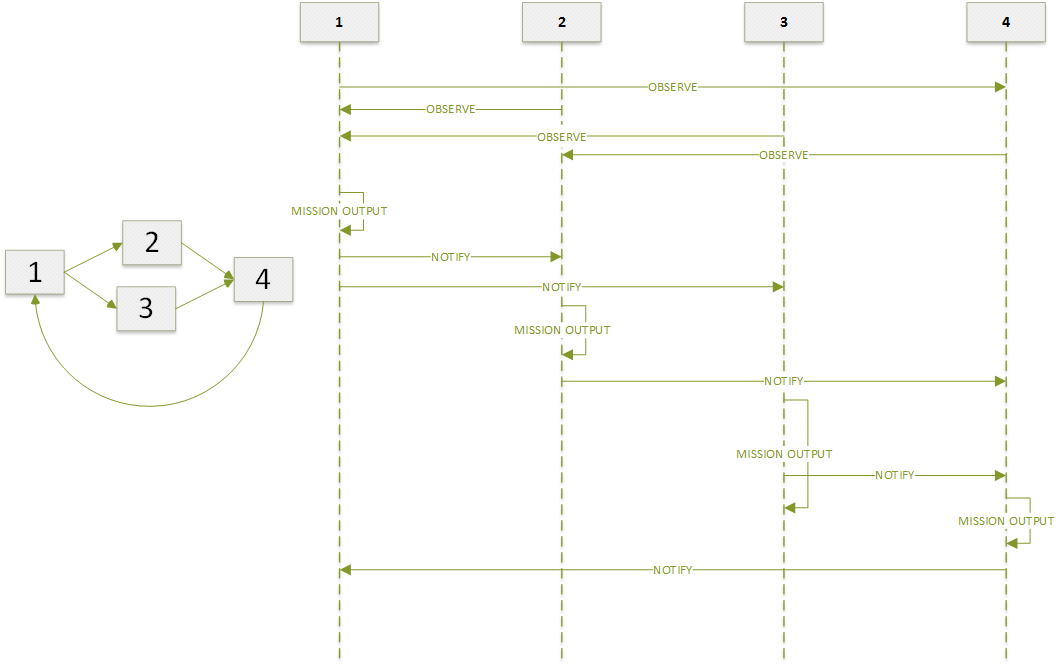
\includegraphics[width=\linewidth]
 {pictures/pub_sub.png}
 \caption{Observer design pattern example}
 \label{fig:observerPattern}
 \end{figure}

In our specific case, we made each declared block of the graphical editor both Observer and Observable. 
This means that each block observes another block that comes before it, but at the same time, it is observed by other blocks coming after it.
\\
The change of status consists in the output of the Mission object.
When a block ends to perform its operations, it notifies all its observers passing them the Mission entity.
\\
For example, in figure \ref{fig:observerPattern} the A block observes the D one; the B and C blocks observe the A and the D observes the B and C both.
\\
So, for example, when the A block ends to modify the Mission object it sends it to the B and C blocks at the same time, which are its observers.
\\

The Editor includes in itself a template model of the Main Application, in which almost all the classes are ready to be executed.
\\
However, this template contains several tags that the generation process will replace with specific lines of code, depending on the drawn graph.
\\
The generation process consists in the search for these tags inside the template application. The tags are:
\\

\begin{itemize}
\item{\textbf{<dec>}: This tag is the placeholder for the code part where the generator engine puts the declaration and the initialization of the entities represented by each blocks.
}
\item{\textbf{<exe>}: This tag is the placeholder for the code part where the generation process declares the Observer pattern. Here the system defines the observers of each blocks depending on the connections in the diagram. 
}
\item{\textbf{<tDelay>}: This tag is the placeholder for a boolean attribute. If the diagram includes the Clock block, this tag will be replaced with a "true" value in order to make the Main Application to ask the user for a delay during the Trip definition.
}
\item{\textbf{<mRep>}: This tag is the placeholder for a boolean attribute. If the diagram includes the Mission Repeater block, this tag will be replaced with a "true" value in order to make the Main Application to ask the user if he wants the Mission to repeat itself.
}
\item{\textbf{<tSafe>}: This tag is the placeholder for a boolean attribute. If the diagram includes the Timer Monitor block, this tag will be replaced with a "true" value in order to make the Main Application to ask the user for a maximum safe time during the Mission creation.
}
\item{\textbf{<tPrt>}: This tag is the placeholder for a boolean attribute. If the diagram includes the Priority Manager block, this tag will be replaced with a "true" value in order to make the Main Application to ask the user for a priority during the Trip definition.
}
\item{\textbf{<num>}: This tag is a placeholder for an integer attribute. If the diagram includes the GateFIFO or GateFunnel blocks, this tag will be replaced by the number of incoming connections of the related Gate block.
}
\item{\textbf{<act>}: This tag is not replaced by the generation process but we need them in order to warn the developer where to insert his Custom Action code.
}
\item{\textbf{<eval>}: This tag is not replaced by the generation process but we need them in order to warn the developer where to insert his custom Evaluator algorithm. 
}
\end{itemize}

\section{Runtime Management}\label{runtimeMng}

The Main Application manages the mission execution with a parallel programming architecture, as shown in figure \ref{fig:threads}.
Indeed when the user starts the execution, the system launches each Mission in a new thread, in order to guarantee a reliable parallel execution.
\\

\begin{figure}[h!]
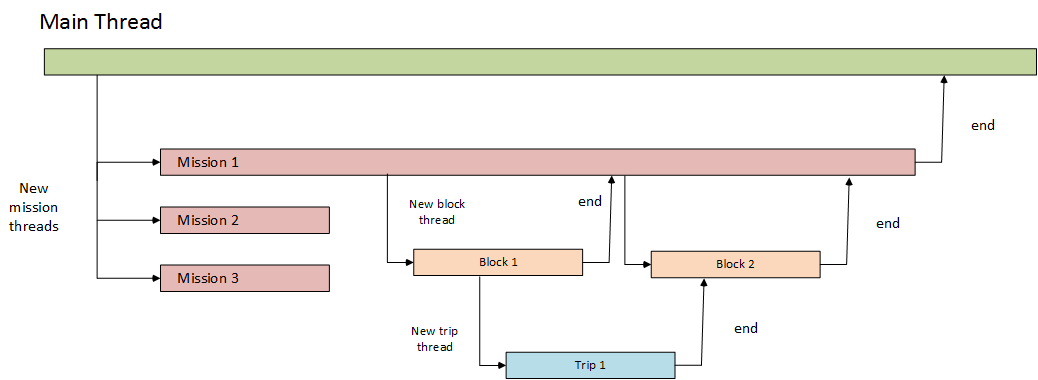
\includegraphics[width=\linewidth]
{pictures/threads.png}
\caption{Example of thread concurrency}
\label{fig:threads}
\end{figure}

Then each mission starts its flow among the blocks, thanks to the Observer design pattern, described in Section \ref{codeGeneration}.
When the mission enters in a new block, the application launches a new thread, in order to run the mission management code of the block.
We need this new thread because there is the possibility that two or more parallel blocks have to manage the same mission entity at the same time.
\\

Therefore, when the mission reaches the "Trip Launcher" block, the system starts the trip.
Doing this, it creates a new thread, to manage the trip execution till its end.
\\

As said, each mission and each trip created by the user, have a respective thread that deal with the execution of the entity from the beginning to the end. In this way, the blocks that need to monitor these entities can observe the status of the threads, in order to know if the trip/mission is still running or has already completed.
\\

It is important to underline that we don't have any synchronization problem among the various threads.
Indeed, there are no dependencies between missions, since each one of them is executed independently from the others.
\\
Inside each Mission entity the trips are executed sequentially:
one trip can start its execution only if the precedent trip in the list has been completed.
\\
Given this independence between missions, the system could dispatch them in a multiple machines cluster. In this way each Mission would run on a different environment maximizing the performance and reducing the load on the single machine.
\\

\section{User interface}\label{interface}

Swing is an advanced GUI toolkit. It has a rich set of widgets:
from basic widgets like buttons, labels, scrollbars to advanced like trees and tables. 
Swing itself is written in Java and is part of JFC, Java Foundation Classes: it is a collection of packages for creating full featured desktop applications.
\\

We used the Swing framework to develop the view part of the MVC pattern shown in section \ref{oomodel},
We needed to develop the three pages of the Pluto Main Application, already described in section \ref{plutoMainApp}, and we knew that Swing provides all the components that we wanted to put in them.
Indeed, since we used it for the development of many academic projects, we noticed that it allows to build graphical interface in a very fast and easy way.

As an illustrative example, figure \ref{fig:tripsPageStructure} shows the structure of the Trips Page:

 \begin{figure}[h!]
 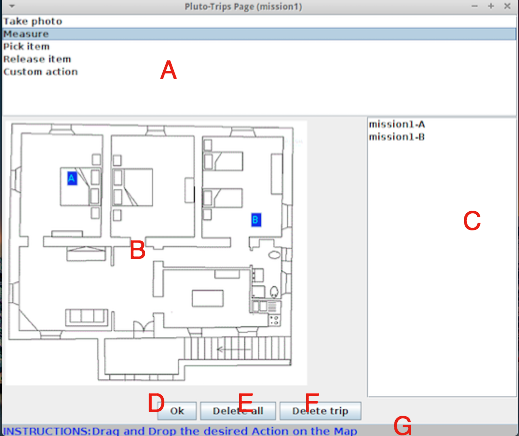
\includegraphics[width=\linewidth]
 {pictures/tripsPageStructure.png}
 \caption{Trips Page structure}
 \label{fig:tripsPageStructure}
 \end{figure}

The Trips Page contains 7 components:

\begin{itemize}
\item {Component A is a \textit{JList}, a list of textual values, in this case the name of the Actions}
\item {Component B is a \textit{JImage}, simply an image representing the Map}
\item {Component C is a \textit{JList}, a list of textual values, in this case the name of the created trips}
\item {Components D,E and F are \textit{JButton}, rectangles that the user can click on}
\item {Component G is a \textit{JTextArea}, an area containing text, in this case the instructions on how to use this page}

All these components are easily usable in Swing, we only needed to import the already provided libraries.
The structure of the other two pages of the Pluto Main Application is very similar to these one, differing only for the contained components.

\end{itemize}


\section{Prototype drone}\label{crazyflie}

For the concrete actuation of the sensing tasks required by each application, we chose the Crazyflie Nano-Quadcopter, shown in figure \ref{fig:crazyflie}.


\begin{figure}[H]
\centering
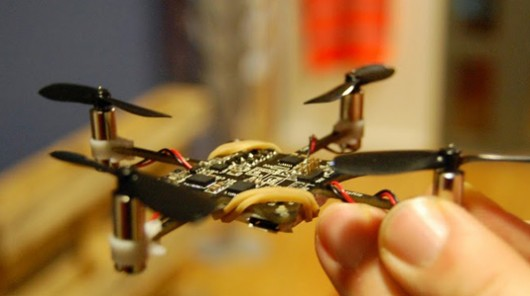
\includegraphics[width=\linewidth]
{pictures/crazyflie.jpg}
  \caption{The Crazyflie Nano-Quadcopter}
  \label{fig:crazyflie}
\end{figure}

The Crazyflie is a tiny quadcopter often referred to as a nano-quad, built using the PCB itself as the frame,developed solely by open source tools. The Crazyflie specs are the following:


\begin{itemize}
\item {Small and lightweight, around 19g and about 90mm motor to motor
}
\item {Flight time up to 7 minutes with standard 170mAh Li-Po battery
}
\item {Standard micro-USB connector for charging which takes 20min for the stock 170mAh Li-Po battery
}
\item {On-board low-energy radio@1mW based on the nRF24L01+ chip. Up to 80m range (environment dependent) when using the Crazyradio USB dongle}
\item{Radio bootloader which enables wireless update of the firmware
}
\item{Powerful 32 bit MCU: STM32F103CB @ 72 MHz (128kb flash, 20kb RAM)
}
\item{3-axis high-performance MEMs gyros with 3-axis accelerometer: Invensense MPU-6050
}
\item{Available footprints to manually solder magnetometer HMC5883L/HMC5983 or/and barometer MS5611
}
\item{4-layer low noise PCB design with separate voltage regulators for digital and analog supply
}
\end{itemize}

We use a particular API that makes the drone move from a \textit{startingLocation} to a \textit{destination} in the environment:
\\

\begin{lstlisting}
	move(startingLocation, destination)
\end{lstlisting}

To concretely control the Crazyflie, there is a Python library which gives high level functions and hides the details.
The precedent API uses the following to send the control commands to the Crazyflie:

\begin{lstlisting}
	send_setpoint(roll, pitch, yaw, thrust)
\end{lstlisting}

The arguments roll/pitch/yaw/trust is the new set-points that should be sent to the copter.
For example, to send a new control set-point:
\\

\begin{lstlisting}
	roll    = 0.0
    pitch   = 0.0
    yawrate = 0
    thrust  = 0
    crazyflie.commander.send_setpoint(roll, pitch, yawrate, thrust)
\end{lstlisting}

Changing the \textit{roll} and \textit{pitch} will make the quadcopter tilt to the sides and thus change the direction that it's moving in.
Changing the \textit{yaw} will make the quadcopter spin.
The thrust is used to control the altitude of the quadcopter.

By dynamically adjusting these four parameters we can make the Crazyflies move to the locations specified by the user through the Pluto User Interface.